\documentclass[11pt,a4paper]{scrartcl}
\typearea{12}
\usepackage{graphicx}
\usepackage{tikz}
%\usepackage{pstricks}
\usepackage{listings}
\usepackage{amsmath}
\usepackage{color, amsfonts}
\usepackage{fancyhdr}
\usepackage{url}
\pagestyle{fancy}
\lfoot{COMS10013 - 2025 - WS4}
\begin{document}

\section*{COMS10013 - Analysis - WS4}

\subsection*{Solutions}


\begin{enumerate}
\item {\textbf{Gradient descent: }} In this question we're going to study the function 
\[E(x,y) = x^2 + y^2\]
\begin{enumerate}
    \item[(a)] $\nabla E(x,y) = (2x,2y)$
    \item[(b)]  We have the  initial value $(x,y) = (1,2)$ and step $\eta = 0.1$.
    \begin{itemize}
        \item $\mathbf{x}_0 = (1,2)$ (because it's just the initial value).
        \item $\mathbf{x}_1 = (1,2) = 0.1\times (2,4)  = (0.8,1.6)$
        \item $\mathbf{x}_2 = (0.64,1.28)$
        \item $\mathbf{x}_3 = (0.512,1.024$
    \end{itemize}
    and $E(\mathbf{x}_3) = 1.3107...$ (to 4 decimal places). Observe the powers of two that arise!
    \item[(c)] Using the same initial value, calculate $\mathbf{x}_0, \mathbf{x}_1, \mathbf{x}_2, \mathbf{x}_3$ taking
    \begin{enumerate}
        \item[(i)] $\eta = 0.5$: we get  $\mathbf{x}_0=\mathbf{x}_1=\mathbf{x}_2= \mathbf{x}_3=(0,0)$. So following the pattern (which one can prove inductively) we get $\mathbf{x}_n = (0,0)$.
        \item[(ii)] $\eta = 1$: we get $\mathbf{x}_0=\mathbf{x}_2= (1,2)$ and $\mathbf{x}_1= \mathbf{x}_3=(-1,-2)$ So following the pattern (that again, we could prove inductively, we get $\mathbf{x}_n = (-1)^n(1,2)$
    \end{enumerate}
    The first choice of $\eta$ is actually (accidentally) a great choice, because (see the next part) it instantly minimises the function. However, it isn't obvious that this is what has happened; for example, we could have hit a local minimum. 
    
    The second choice of $\eta$ is definitely poor: we're flipping between two values, rather than `honing in' on the minimal solution. 

    \item[(d)] Find all minima of $E$ using calculus: First of all, we'll find the critical points of $E$ by looking at $\nabla{E}$: if $\nabla{E} = (0,0)$, then $x= y = 0$. This is the only critical point; now we can argue that $(0,0)$ is a minimum by using the fact that $x^2 + y^2 \geq 0$, and $E(0,0) = 0$.
    
    \item[(e)] Pick a new initial starting point (not a minimum value that you found in (d)!), and calculate $E(\mathbf{x}_3)$ using $\eta = 0.1$. Compare this to what you found in (b) -- is it a better starting point? 
    Is this what you'd expect given what you found in (d)?
   \\
   For example, let's pick the initial starting point $(5,8)$. A couple of rounds of this gives $E(\mathbf{x}_3) \approx 23$, which is further from the minimum than the results from $(c)$ -- this makes it a worse initial starting point. This isn't hugely surprising because this point is further away from the actual minimum than $(1,2)$, and we're using a very symmetric function with the same value of $\eta$. If our function of choice were less regular, then the distance from the actual minimum wouldn't necessarily matter so much.
\end{enumerate}

\newpage
\item \textbf{Nelder-Mead Method:} In this question, we're going to study the function 
\[
    E(x,y) = x^2 + y^2\,.
\]
The eagle-eyed amongst you will notice that this is the same function as in question 1. This means that we already know what the minimum should be; the purpose of this question is to use the downhill simplex method to find the minimum. 

We'll start with the initial simplex points: $(0,0), (1,0), (0,1)$.
\begin{enumerate}
    \item[(a)] Draw the initial simplex and assign values $\mathbf{x}_1, \mathbf{x}_2, \mathbf{x}_3$ to the initial simplex points so that $E(\mathbf{x}_1)\leq E(\mathbf{x}_2) \leq E(\mathbf{x}_3)$. \\
    
\begin{tikzpicture}
    \tikzstyle{point}=[thick,draw=black,cross out,inner sep=0pt,minimum width=4pt,minimum height=4pt]
    \draw (0,0) node[anchor=north]{$\mathbf{x}_1 = (0,0)$}
      -- (4,0) node[anchor=north]{$\mathbf{x}_2 = (1,0)$}
      -- (0,4) node[anchor=south]{$\mathbf{x}_3= (0,1)$}
      -- cycle;
\end{tikzpicture}
Since $E(\mathbf{x}_2) + E(\mathbf{x}_3)$, it's equally correct to have swapped the assignment of these two values. 
    
    \item[(b)] The centroid is given by 
    \[
        \mathbf{x}_0= \frac12 \left(
        \begin{pmatrix}
        0\\0
        \end{pmatrix}
        + 
                \begin{pmatrix}
        1\\0
        \end{pmatrix} \right)= 
        \begin{pmatrix}
        \frac12\\0
        \end{pmatrix}        
    \]
    If you had the other assignment of the $\mathbf{x}_2$ and $\mathbf{x}_3$ variables, then the centroid is instead given by $\begin{pmatrix}
        0\\\frac12
    \end{pmatrix}$.

    The reflection point $\mathbf{x}_r$ is 
    \[
    \mathbf{x}_r = \mathbf{x}_0 + (\mathbf{x}_0 -\mathbf{x}_3) = 
    \begin{pmatrix}
        1\\0
        \end{pmatrix}-
        \begin{pmatrix}
        0\\1
        \end{pmatrix}        
         =
         \begin{pmatrix}
        1\\-1
        \end{pmatrix}        
    \]
    Hence $E(\mathbf{x}_r) = 2$. 
    \item[(c)] Notice that $E(\mathbf{x}_r)$ is a worse outcome in terms of this minimisation outcome (i.e. it gives a bigger output). This is bad! We won't proceed using this new point -- instead the algorithm tells us to find a contraction point:
    \begin{align*}
     \mathbf{x}_c &= \mathbf{x}_0 - \frac12 (\mathbf{x}_0 -\mathbf{x}_3) \\
     &= 
    \begin{pmatrix}
        \frac12 \\0
        \end{pmatrix}-\frac12\left[
        \begin{pmatrix}
        \frac12 \\0
        \end{pmatrix}       
        - 
        \begin{pmatrix}
        0\\1
        \end{pmatrix}       
        \right]\\
         &=
         \begin{pmatrix}
        \frac14\\\frac12
        \end{pmatrix}   \,.  
    \end{align*}
    Now $E(\mathbf{x}_c) = \frac1{16} + \frac1{4} = \frac5{16}
$, so our output has (as desired) decreased. This means our new point is    $      \begin{pmatrix}
        \frac14\\\frac12
        \end{pmatrix}$.

Let's have a look at our new simplex:\\

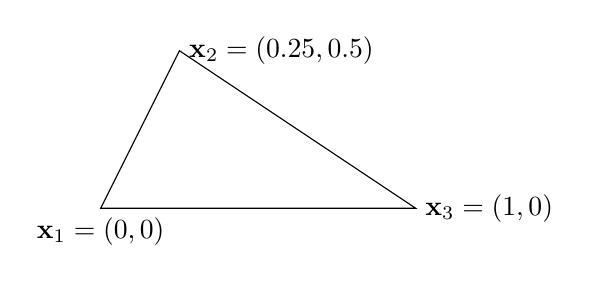
\begin{tikzpicture}
    \tikzstyle{point}=[thick,draw=black,cross out,inner sep=0pt,minimum width=4pt,minimum height=4pt]
    \draw (0,0) node[anchor=north]{$\mathbf{x}_1 = (0,0)$}
      -- (1,2) node[anchor=west]{$\mathbf{x}_2 = (0.25,0.5)$}
      -- (4,0) node[anchor=west]{$\mathbf{x}_3= (1,0)$}
      -- cycle;
\end{tikzpicture}

        \item[(d)] The subsequent centroid is $      \begin{pmatrix}
        0.125\\0.25
        \end{pmatrix}$ and the next $\mathbf{x}_r$ value is $      \begin{pmatrix}
            -0.75\\0.5
        \end{pmatrix}$.
        Thus $E(\mathbf{x}_r) - 0.8125$, which is less than $E(\mathbf{x}_3)$, so we'll swap in $\mathbf{x}_r$:

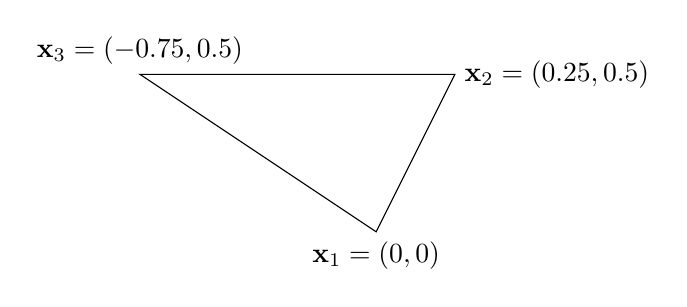
\begin{tikzpicture}
            \tikzstyle{point}=[thick,draw=black,cross out,inner sep=0pt,minimum width=4pt,minimum height=4pt]
    \draw (0,0) node[anchor=north]{$\mathbf{x}_1 = (0,0)$}
      -- (1,2) node[anchor=west]{$\mathbf{x}_2 = (0.25,0.5)$}
      -- (-3,2) node[anchor=south]{$\mathbf{x}_3= (-0.75,0.5)$}
      -- cycle;
\end{tikzpicture}

Let us continue:\\
the next centroid is still $(0.125,0.25)$. The next reflection point is 
\[
(0.25,0.5) - (-0.75, 0.5) = (1,0);
\]
this is a familiar point and would result in us going in a circle. The algorithm tells us to turn to a contraction point again:
\[
\mathbf{x}_c = \begin{pmatrix}
        0.125\\0.25
        \end{pmatrix}
     -
     \frac12 \left(
     \begin{pmatrix}
        0.125\\0.25
        \end{pmatrix}
        - \begin{pmatrix}
        -0.75\\0.5
        \end{pmatrix}
     \right)
     = 
     \begin{pmatrix}
         -0.3125\\ 0.375
     \end{pmatrix}
\]
and $E(\mathbf{x}_c) = 0.223828125$.

So our contraction point becomes a new point in our simplex:

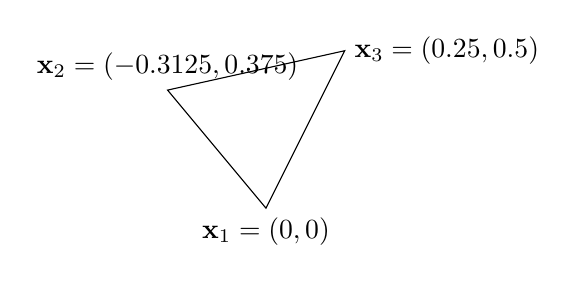
\begin{tikzpicture}
            \tikzstyle{point}=[thick,draw=black,cross out,inner sep=0pt,minimum width=4pt,minimum height=4pt]
    \draw (0,0) node[anchor=north]{$\mathbf{x}_1 = (0,0)$}
      -- (1,2) node[anchor=west]{$\mathbf{x}_3 = (0.25,0.5)$}
      -- (-1.25,1.5) node[anchor=south]{$\mathbf{x}_2= (-0.3125,0.375)$}
      -- cycle;
\end{tikzpicture}

    \item[(e)] In this picture, we're iteratively swapping out either $\mathbf{x}_2$ or $\mathbf{x}_3$ until the simplex (i.e. the triangle) gets closer to the point $(0,0)$. Because $\mathbf{x}_1$ is the actual minimum, we won't touch it when creating new points. 

    A sensible stopping condition might be after a certain number of steps, or when then rate of change of the $E(\mathbf{x}_0)$ (the centroid at a given iteration) begins to slow.  

    These suggestions are by no means exclusive. 
    
\end{enumerate}
\end{enumerate}

\subsection*{Extra questions}

These are extra questions you might attempt in the workshop or at a later time. Some parts of these questions require a computer (e.g. using Python).

\begin{enumerate}
\item \textbf{Gradient descent: } In this question we're going to aim to minimise the function 
\[
f(x,y) = e^{-x}\cos(x) y^2
\]
using Gradient descent.

\begin{enumerate}
    \item[(a)] $\nabla f(x,y) = (-e^{-x}\cos(x) y^2 - e^{-x}\sin(x)y^2, 2e^{-x}\cos(x)y)$
    

    \item[(b-d)] 'Solutions' on this depend very much on what you've picked. Here's some code that I used in Python:
    \begin{verbatim}
import math

def grad(x,y):
    return [-math.exp(-x)*math.cos(x)*pow(y,2)-math.sin(x)*math.exp(-x)*pow(y,2),
           2*math.exp(-x)*math.cos(x)*y]

vec = [1,2] # your random vector here

eta = 0.01
#eta = 0.1
#eta = 0.5

iters = 0
limit = 100

while iters < limit:
    [x,y] = [vec[0],vec[1]]
    newgrad = grad(x,y)
    vec = [x - eta*newgrad[0], y - eta*newgrad[1]]
    iters += 1
    print(iters, vec, math.exp(-x)*math.cos(x)*y**2) # prints i, x_i, , f(x_i)
        
    \end{verbatim}
    
    \item[(e)] Look again at $f$; what do you expect the minimum value to be? \\
    To minimise $f$, we want to take $x$ and $y$ to make it as  negative as possible; $e^{-x}$ and $y^2$ are always positive, so we're going to have to take $x$ so that $\cos(x)$ is as negative as possible - this means that $\cos{x}=-1$. Now we can take $y\to \infty$, so we get $f(x,y) = -\infty$. Outputs from (c) and (d) should aim to therefore be as small and as negative as possible; a good performance would be going quickly towards this minimum value. 
\end{enumerate}

\item \textbf{Nelder-Mead: } 
There are no `sample' solutions here because there's a myriad of ways that you could implement this and seeing a method that isn't yours isn't hugely helpful. Feel free to discuss your solution in person. 

\end{enumerate}

\end{document}
